% !TEX encoding = UTF-8 Unicode
% !TEX root = SystemTemplate.tex

\documentclass{book}
\input{seniordesignstyle.tex} % This sets the format.

% Add your title page contents here 
\title{{\color{MSBlue1} \rule{\linewidth}{0.5mm}}\\[2mm] {\huge \bfseries \color{MSBlue1} Automatic Program Tester }\\[-1mm] {\color{MSBlue1}\rule{\linewidth}{0.5mm}} \\  \vfill
{\LARGE \bfseries \color{MSBlue2} Software Engineering Spring 2014  Documentation }\\  \vfill 
{\color{MSBlue1} Sprint 1: We Can't Follow Directions} \\
{\color{MSBlue2} Sprint 2: Software Engineering Adventure Line} \\
{\color{MSBlue3} Sprint 3: Lounge Against the Machine}}
\author {
\color{MSBlue1} Sam Carroll \and \color{MSBlue1} Colter Assman \and \color{MSBlue1} Shaun Gruening \and
\color{MSBlue2}  Erik Hattervig \and \color{MSBlue2} Andrew Koc \and  \color{MSBlue2} Jonathan Tomes \and 
\color{MSBlue3}  Joe Manke \and \color{MSBlue3} Adam Meaney}
\date{\color{MSBlue1} \today}


\begin{document}
\frontmatter
\maketitle

\tableofcontents
\listoffigures
\listoftables
\listofalgorithms

% !TEX root = SystemTemplate.tex

\chapter{Mission}

To lounge as much as possible while producing quality software.  % add mission statement to mission.tex
% !TEX root = SystemTemplate.tex

\chapter{Document Preparation and Updates}

Current Version [3.0.0]
\vspace*{5mm}

{\color{MSBlue3}
\noindent
\textit{Prepared By:}\\
\textit{Sam Carroll}\\
\textit{Colter Assman}\\
\textit{Shaun Gruenig}\\
\textit{Erik Hattervig}\\
\textit{Andrew Koc}\\
\textit{Jonathan Tomes}\\
\textit{Joe Manke}\\
\textit{Adam Meaney}\\
}

\vfill
\noindent
{\color{color02} \textit{\textbf{Revision History}}}\\
\begin{tabular}{|>{\raggedright}p{1.5cm}|>{\raggedright}p{3cm}|>{\raggedright}p{1.5cm}|>{\raggedright}p{9cm}|}
\hline
\textit{\textbf{Date}} &  \textit{\textbf{Author}} & \textit{\textbf{Version}} & \textit{\textbf{Comments}}\tabularnewline
\hline
 \textit{\textbf{2/19/14}} & \textit{Samuel Carroll} & \textit{1.0.0} & \textit{Initial version}\tabularnewline
\hline
 \textit{\textbf{3/23/14}} & \textit{Jonathan Tomesl} & \textit{2.0.0} & \textit{Sprint 2 Version}\tabularnewline
 \hline
 \textit{\textbf{4/27/14}} & \textit{Joe Manke} & \textit{3.0.0} & \textit{Sprint 3 Version}\tabularnewline
\hline
\end{tabular}
\vfill



\mainmatter

%%  Add to the following chapters

% !TEX root = SystemTemplate.tex

\chapter{Overview and concept of operations}

This document will look at the Lounge Against the Machine team's third sprint for building
a program tester. Looking at the team members and their roles, the project
management that we used, the sprint retrospective, any terminology or acronyms
that we use. Next we will look at the user stories, backlog and requirements of the
program. Then we will look at the design and implementation of the program focusing
on major pieces of the code. The next section will look at system and unit testing of 
our program, followed by development environment, and release, setup and
deployment of our program. We will finish this document with a look at a user 
documentation (including a user guide, installation guide and programmer manual)
class index and class documnetation.


\section{Scope}
This document will cover the third sprint of our program tester built for Dr. Logar's
software engineering class in Spring 2014 .


\section{Purpose}
The purpose of this program is to compile, run and test the simple programs created by others. The program willl also offer to generate additonal random tests.

\subsection{Normal Run}
The programs it tests are guaranteed to compile and run correctly. It will then search through a root directory, find each student's
subdirectory, compile their code into the root directory, open log files for the student and the class as a whole. Student logs will
go into the student's directory and the class log will be in the root. The student logs will have the results of each test, a final
score, and results from running GNU tools gprof and gcov on the program. The final score will be based on the precent of the tests passed. A program may be marked as a fail if it fails a critical test, or times out. Critical tests are labeled as "crit\_(something).tst".

\subsection{ Generate Tests}
The program will ask for a number tests to generate, the number of inputs for
each test, and the data type for the tests. The program will then generate a "GeneratedTests" directory in the test directory of the root
folder. At which point, the program will generate the number of tests specified. If the program has previously generated tests, it will
then remove the past generated tests and create new ones. 


\section{Systems Goals}
1) Find student programs to compile.\\
2) Find the tests and use them to test the found programs.\\
3) Generate new random test cases.\\
4) Log information about the test runs, including pass percentage, code coverage, and code performance.

\section{System Overview and Diagram}
The program will be started on the command line. You may specify a testing directory. If a testing directory is not supplied, the program will assume its current directory is the testing directory. It will then display a simple menu for executing existing test cases, generated new test cases, or exiting.  See Figure~\ref{systemdiagram}.

\begin{figure}[tbh]
\begin{center}
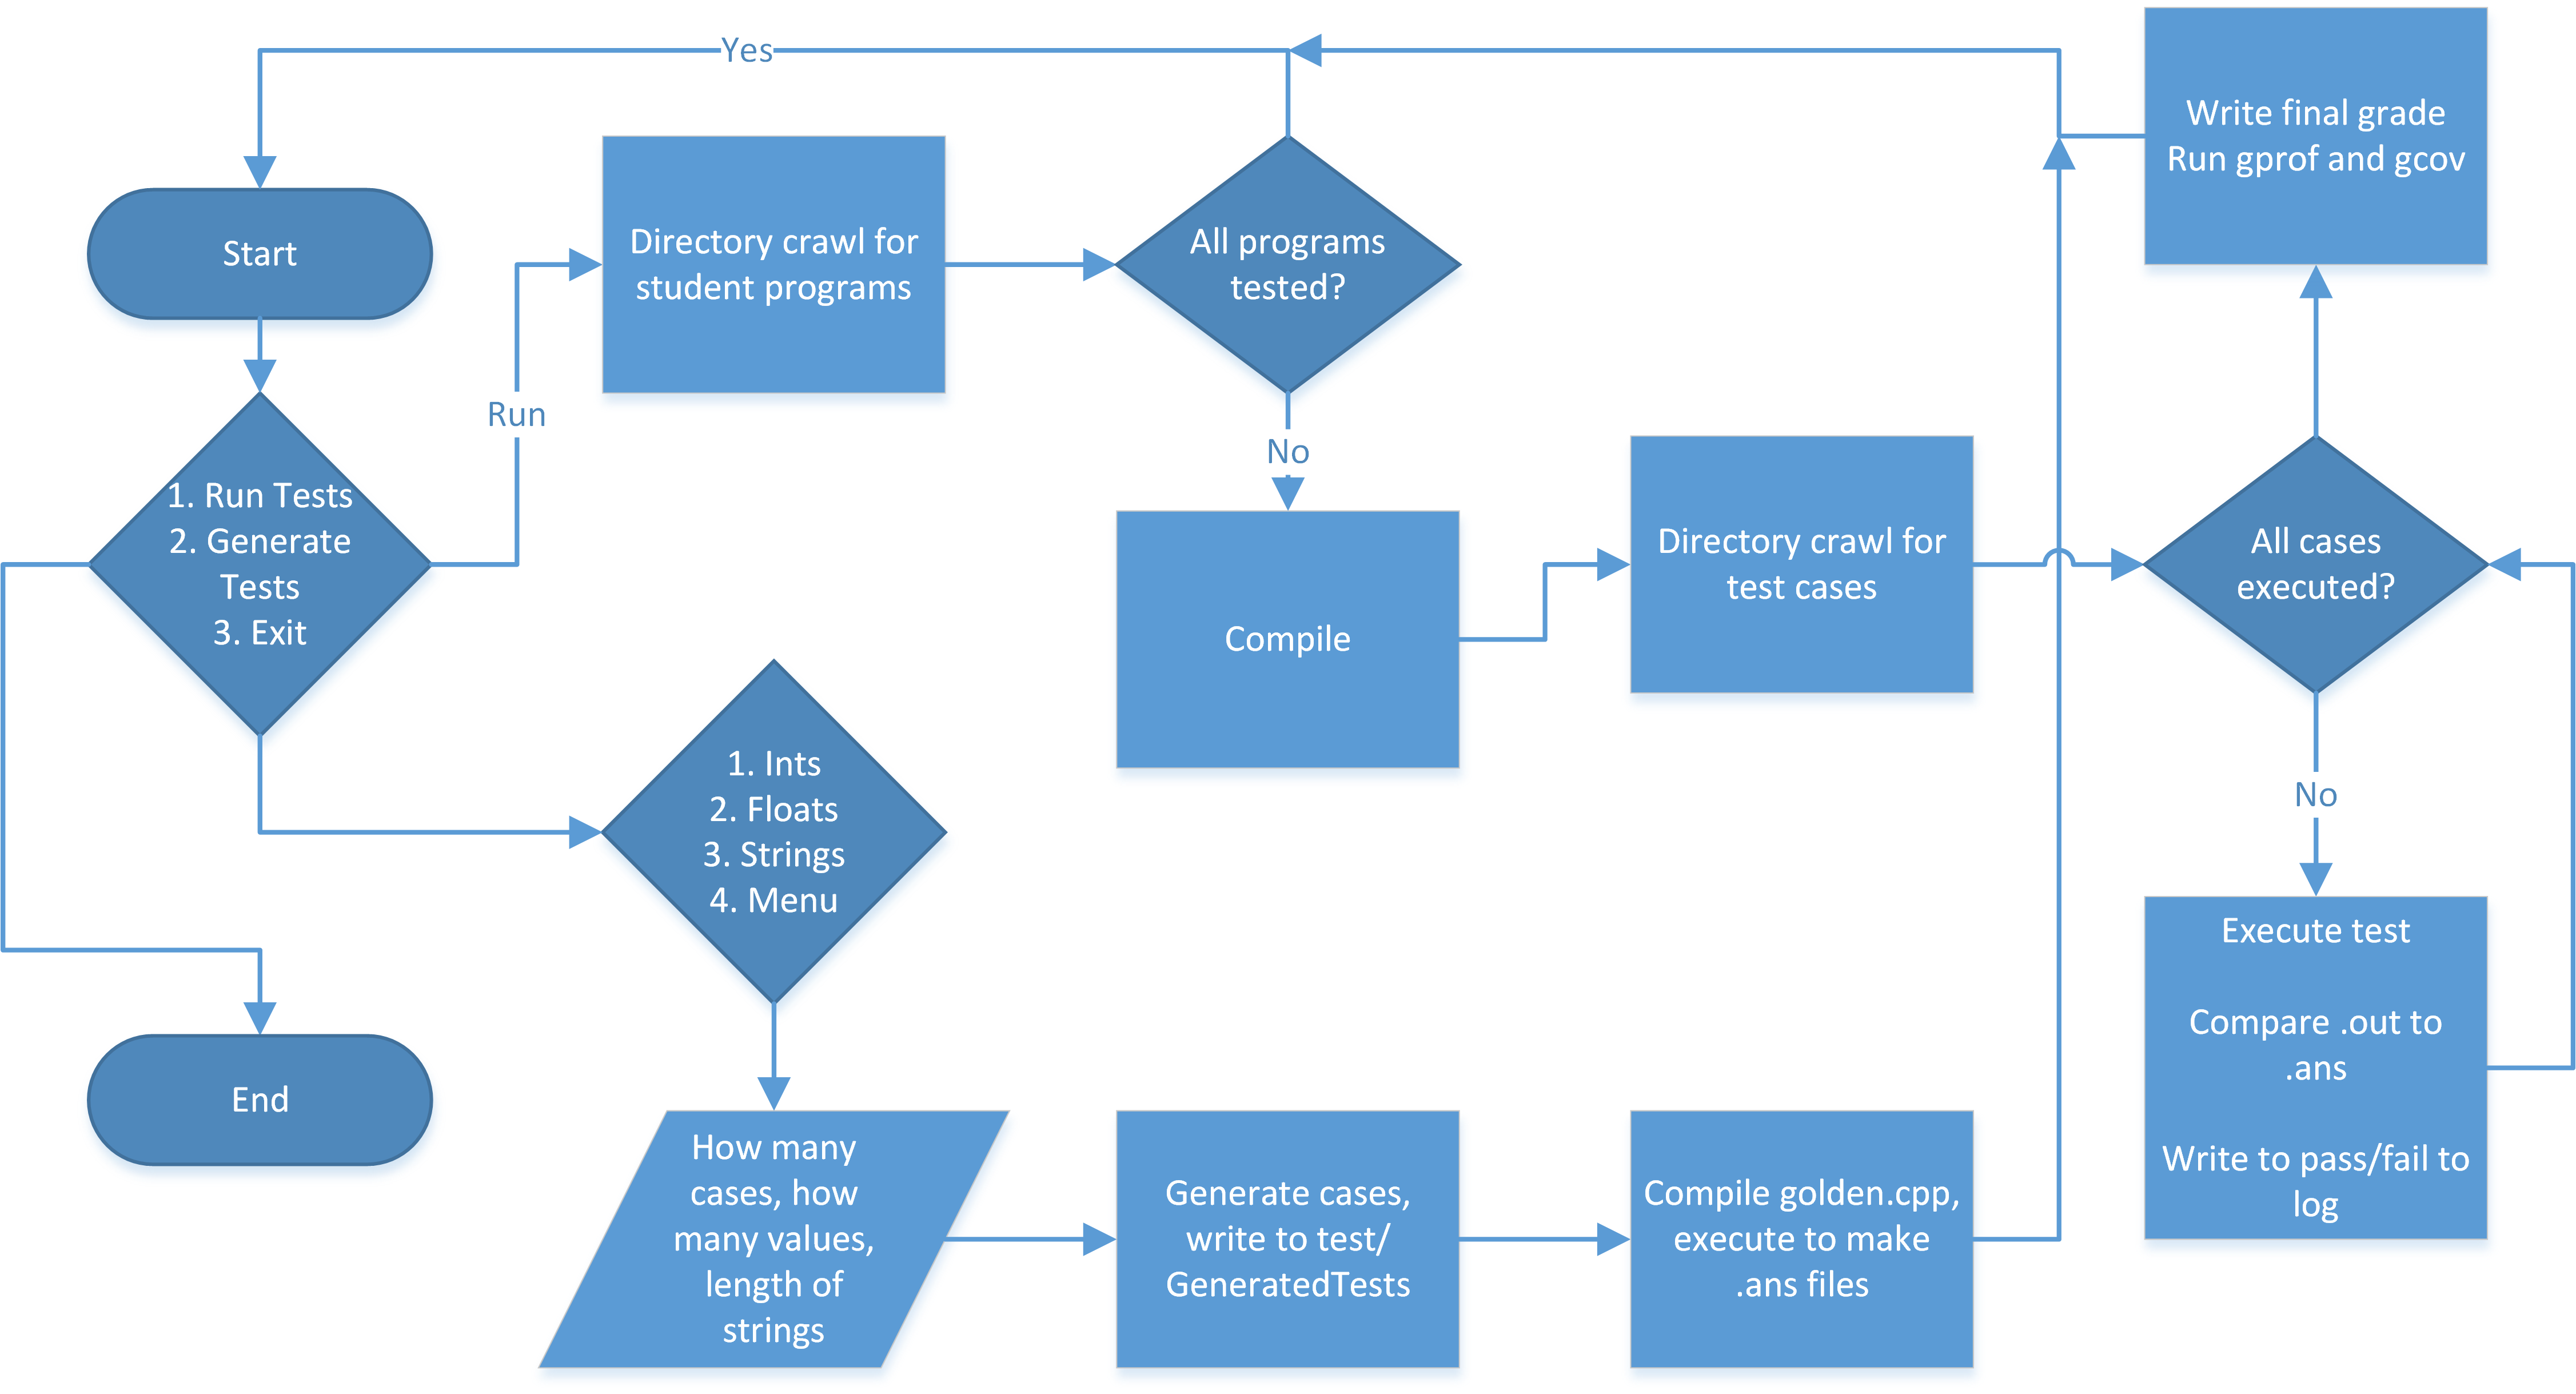
\includegraphics[width=0.75\textwidth]{./SystemDiagram}
\end{center}
\caption{System Diagram \label{systemdiagram}}
\end{figure}

\section{Technologies Overview}
The program was written in C++, and was compiled with g++ on a linux environment. The program also requires use of GNU tools gprof and gcov. Project management was done through Trello. Source control was done through GitHub. Documentation was created using \LaTeX.

% !TEX root = SystemTemplate.tex


\chapter{Project Overview}
This section provides information regarding the team and their roles,
how the project was managed, and any relatively unkown terminology or
acronyms.



\section{Team Members and Roles}
For Sprint 1, the team members were:\\
\indent Product Owner: Sam Carroll\\
\indent Scrum Master: Colter Assman\\
\indent Technical Lead: Shaun Gruenig\\ \\
For Sprint 2, the team members were:\\
\indent Product Owner: Erik Hattervig \\
\indent Scrum Master: Jonathan Tomes\\
\indent Technical Lead: Andrew Koc\\ \\
For Sprint 3, the team members were:\\
\indent Product Owner: Joe Manke\\
\indent Scrum Master: Adam Meaney\\
\indent The team members shared duties as Co-Techical Leads.


\section{Project  Management Approach}

The program was created using the Scrum Agile Approach.
The sprint length for this project was 2 weeks. We began with a meeting to
decide the user needs and split the program accordingly. Each of us would code
different parts of the program and then we would all test and re-code as needed.

Cards were created on Trello to keep track of tasks, and a repository was created on GitHub for the code.

\section{Phase  Overview}
Sprint 1 (We Can't Follow Directions):

This program started in a gathering information phase, the first thing we had to do as a team 
was generate several questions to ask the customer (Dr. Logar) about the software that she 
wanted.   The next phase was asking if it could be done, as most of the code had been written 
at one point or another for our team, we decided that it was a program that could be written.  
The next phase was breaking the program into smaller milestones, we decided that the program 
would need to compile source code, search for test cases, run compiled code with test case, 
output test case results to a file, compare that output file to an expected output file, and then 
write to a file if the two files match or not, if they do we write the text case then passed to a log 
file, if they don't we write the text case and failed to the log file.   Once we are done traversing the 
directory we write the total number of passed, failed and percentages of each. \\

Sprint 2 (The Software Engineering Adventure Line):

First we began with an information gathering session by Dr. Logar and the product owners. This is where we
found out the goals of the program and the desired results. After this we were assigned a team's work
from the previous sprint, and evaluted it. Unfortunately we had to do a lot of revising and creating new
functions because the old cold was not very modular. So we divided up the work of reworking the code and
did our parts. After that we gathered and came up with how to meet the new requirements and worked out
what we needed to code, ask the user for, and finished coding the program. \\

Sprint 3 (Lounge Against the Machine):

Information gathering was done in-class with Dr. Logar. During this class session, we were assigned the code from the team Adventure Line. A short code review ensued where we initially had issues with the directory setup. We were also given non-compiling \LaTeX files instead of a PDF, which made documentation review difficult. After these small issues were straightened out, we divided up tasks for the sprint. Then we began adding to the existing code base to add the new functionality. Since we did not perform a very thorough code review, we did not discover a few issues of code efficiency until too late in the development cycle to fix them. Specifically, we realized that the program re-searches for all test cases for every tested program, instead of finding test cases once and storing their paths. 

\section{Terminology and Acronyms}
N/A

% !TEX root = SystemTemplate.tex
\chapter{User Stories, Backlog and Requirements}
\section{Overview}

This section will look at the userstories of the development of the program, the requirements
of the program, the proof of concept results, and research task results. It will also look at the
reason for developing this software. 

\subsection{Scope}

This document will contain stakeholder information, 
initial user stories, requirements, proof of concept results, and various research 
task results. 

\subsection{Purpose of the System}
To test a set of basic computer programs written in the C++ language so a grade can quickly be assigned to a class of students.
The system will also be able to generate random test cases from user input.

\section{ Stakeholder Information}

The people most interested in this project is Dr. Logar and perhaps other computer science faculty, who are looking to quickly
and easily, grade programs that are turned in by CSC 150 students.

\subsection{Customer or End User (Product Owner)}
The product owner on the first sprint was Samuel Carroll, he created a list with his teammates 
and on a day, selected by Dr. Logar, met with her and the other teams' product owner to determine
exatly what Dr. Logar wanted. Samuel was also the team member most involved in keeping the Trello 
board up to date.

The product owner on the second sprint was Erik Hattervig, he gathered the necessary requirments of the
second sprint from Dr Logar, relaied the information to his teammates, and set up the product backlog on
the Trello board.

The product owner on the third sprint was Joe Manke. He gathered requirements from Dr. Logar, created the cards on Trello, and set up the GitHub repository for the sprint.

\subsection{Management or Instructor (Scrum Master)}
The scrum master for the first sprint was Colter Assman, his duties were to ensure that the project 
stayed on track and if any team member ran into some issues he would help them get back on track.   
Colter also was responsible for the running of the daily scrum.

The scrum master for the second sprint was Jonathon Tomes,  he was in charge of managing the scheduling
for the team members, creating spring schedules, and moving tasks from the product backlog to the sprint backlog.
He also lead the scrum meetings.

The scrum master for the thrid sprint was Adam Meaney. He assigned tasks and managed the Trello board.

\subsection{Investors}
Our sole investor is Brian Butterfield, who will be reviewing all teams' products and awarding one team the Butterfield Cup for Excellence in Software Engineering, also colloquially known as the Buttercup.

\subsection{Developers --Testers}
Shaun Gruenig was the biggest tester for our program.   As the team technical lead 
he kept us updated on if the project was running as we expected it to, and would 
often debug the issues our code had.

For the second sprint, all three members of the team tested each other's code and gave feed back on bugs and
code quality via Github.

For the third sprint, both members of the team shared development and testing responsibilities, though Adam Meaney did more of the testing.

\section{Business Need}
Currently many computer science teachers have to write each test case out by hand.   
This is a very time consuming endeavor (especially considering how many students each
one has), so this program would enable them to write a test cases which will then be input
to our program. This program's purpose is to help teachers quickly and accurately assign grades to students.

\section{Requirements and Design Constraints}
The requirements are that the program be written in C++ and work in a Linux environment. Dr. Logar also required the use of Trello and GitHub for product management, and for documentation to be written with \LaTeX.


\subsection{System  Requirements}
The program must be able to run on a Linux machine, using the GNU operating system.   
therefore the code must able to compile using the GNU compiler.   This means all of our
code must be executable on Linux machines.

\subsection{Development Environment Requirements}
Linux/GNU system should be able to run our tester. 


\subsection{Project  Management Methodology}
The stakeholders had several requests on how the project was implemented. Including 
what to use to keep track of backlogs and sprint status, which parties had access to the
sprint and produt backlogs, how many sprints will be used for this project, and restrictions
on the source control.
 
\begin{itemize}
\item Trello was used to keep track of the backlogs and sprint status
\item All parties will have access to the Sprint and Product Backlogs
\item Three sprints will encompass this project
\item The sprints will vary in length a little bit but be about 2-3 weeks in general
\item Github was used for source control
\end{itemize}

\section{User Stories}

\subsection{Sprint 1}

\subsubsection{Compile and Run Source Code}
The program must be able to compile and run source code found in the directory.

\subsubsection{Write Pass/Fail and Percentages to Log File} 
This program must be able to write output to a log file and to keep track of the total number
passed cases and the total number of failed cases.

\subsubsection{Compare Output with Expected Output}
The program must be able to compare the output that we get after running a test case to the
output that we expect to get from the test case. The expected output will be found when 
searching the directory.

\subsubsection{Searching/Traversing the Directory}
The program must be able to search through all the files and sub-directories of the directory 
that we are currently in.

\subsubsection{Invoking the Program}
The user must be able to run our program by typing "./test directoryName" from the terminal.

\subsection{Sprint 2}

\subsubsection{Class Testing}
The user should be able to run tests against an entire class's programs at once.

\subsubsection{Test Case Generation}
The user should be able to generate test cases with randomly generated integers or floating-point numbers.

\subsubsection {Acceptance Testing}
The user should be able to designate test cases as critical, and mark a program as a failure if it does not pass these tests.

\subsection{Sprint 3}

\subsubsection{Infinite Loop Detection}
The program should be able to detect an infinite loop and halt program execution.

\subsubsection{Presentation Errors}
The program should be more lax in output comparison, and allow a pass with presentation errors.

\subsubsection{Expanded Test Generation}
The user should be able to generate test cases for strings and menu-driven programs.

\subsubsection{Performance Testing}
The program should log performance statistics for tested programs using the GNU tool gprof.

\subsubsection{Code Coverage}
The program should log code coverage statistics for tested programs using the GNU tool gcov.

\section{User Story Breakdowns}
\subsection{Sprint 1}

\subsubsection{Compile and Run Source Code}
The program compiles tested programs using the GNU g++ compiler. Compilation and execution are achieved using system commands.

\subsubsection{Write Pass/Fail and Percentages to Log File} 
Each test case is given a pass/fail grade per program, based on output comparison. The final grade for a program is the percentage of test cases passed. In Sprint 2, critical failures were introduced. In Sprint 3, passes with presentation errors were introduced.

\subsubsection{Compare Output with Expected Output}
For each test case, output is redirected to a .out file. This file is compared to a .ans using the diff command. For Sprints 1 and 2, the .out file must be identical to the .ans file for a program to pass a test case. In Sprint 3, looser requirements were introduced allowing a pass with presentation errors.

\subsubsection{Searching/Traversing the Directory}
The program performs recursive directory crawls starting in the given directory to find test cases, notated by a .tst extension, and test source code with .cpp extensions. In Sprint 2, this was modified so all test cases should be in a directory named "test", but may be located in child directories of that. Also as of Sprint 2, test source code for each student should be in a directory with the same name as the .cpp file (i.e. directory "student1" contains "student1.cpp").

\subsubsection{Invoking the Program}
The user must be able to run our program by typing "./test directoryName" from the terminal. This executable name is guaranteed by compiling the program using the provided makefile.

\subsection{Sprint 2}

\subsubsection{Class Testing}
The executable should be located in a class directory. This directory should contain a directory named "test" where all test cases are located, and individual directories for each student. When tests are executed, a class log file sharing the name of the directory is written in the top level directory, and each student has an individual log file placed in their directory. The class log contains the final grade for each student.

\subsubsection{Test Case Generation}
When the program is started, the user is presented with a menu to either run existing test cases or generate new test cases. When generation is selected, the user is prompted for what type of data to generate. In Sprint 2, this was limited to integers and floats. Then, the user is asked how many cases to generate, and how many values to put in each test case. With this information, the program randomly generates values between 0 and 1000 and writes them to files named Test\_X.ans, located in the directory "test/GeneratedTests". This directory will be created anew every time test cases are generated. 

After the test cases have been written, .ans files are created using a .cpp file located in the starting directory. This program is compiled and tested against each generated test case, with the .ans files also stored in "test/GeneratedTests". The user is then returned to the starting menu, allowing them to run their newly made test cases.

In Sprint 3, this was expanded to include strings and menus.

\subsubsection {Acceptance Testing}
Tests with filenames of "x\_crit.tst" are considered critical or acceptance tests. If a program does not pass all critical test cases, it is considered a failure regardless of the percentage of non-critical tests it passes. Critical tests are not included in the final grade percentage.  

\subsection{Sprint 3}

\subsubsection{Infinite Loop Detection}
This is not an attempt to solve the halting problem. Tested programs are now run in a forked child process, and killed if they do not complete within a given time. The user is asked if they want to adjust the timeout limit from its default of 60 seconds when they choose to run tests. If the program does not finish on its own before the timeout, it is considered a critical fail.

\subsubsection{Presentation Errors}
Tested programs are now allowed to pass without their .out file being exactly identical to the .ans file for the test case. There are five allowed presentation errors:
\begin{itemize}
\item Whitespace differences
\item Case sensitivity
\item Correct first and last letters, incorrect internals (e.g., "Definitely" vs "Definently") 
\item Letters in incorrect order (e.g., "Option" vs "Optoin")
\item Floating point values: If the .out file has more precision than the .ans file, but rounds up to the number in the .ans file, it is correct. If the .out file is less precise than the .ans file, it is incorrect.
\end{itemize}

Test cases which differ only on presentation are notated as "Passed with presentation errors" in the log file.

\subsubsection{Expanded Test Generation}
The program can now generate test cases using strings or designed for menu-driven programs.

For strings, selecting the number of cases and values to generate is the same as for integers and floating-point values. In addition, the user selects if the strings should all be the same length or variable. The user then specifies a (maximum) length for the strings, capped at 80. All strings consistent only of lowercase letters encoded in ASCII.

For menus, the user only specifies how many test cases to create. The number of values per test case is determined a .spec file, located in the root directory. The format of each line of the .spec file is the menu option (an integer) then either "int" or "double" for every value to be generated. These values will not be bounded. \\
Example: The line "1 int int double" in a .spec file couldl generate the line "1 4095 728294 8374.837" in a .tst file.

\subsubsection{Performance Testing}
The test programs are compiled with the -pg flag so that they may be profiled using gprof. After the program is tested, the command "gprof studentName > studentName.gprof" is executed, writing the full flat profile to a file named studentName.gprof in the student's directory. The name of each function and its percentage of runtime are also written into the student's log file.

\subsubsection{Code Coverage}
The test programs are compiled with the flags "-fprofile-arcs -ftest-coverage." After the program is tested, the command "gcov studentName" is executed, creating a file named "studentName.gcov" in the student's directory. The code coverage is also reported in the student's log file.

\section{Research or Proof of Concept Results}
Most of the code had been written by our team before.   We knew how to run the system 
function in C++ to invoke a system command. We had built a directory crawler in an earlier 
class (though in Windows so some modification had to take place).   All in all starting the 
program we knew we could complete it.

For Sprint 2 much of the same concepts applied for the new features that were added such as
test case generation.

For Sprint 3, gprof and gcov had to be researched, but the rest of the new features were rather simple.

\section{Supporting Material}

In the man pages for the diff function it shows us that it returns one of three values and 
the case those values are returned, a zero if there is no difference between the two files, 
a one if there is a difference between the two files, or a two if something went wrong (doesn't happen often)


% !TEX root = SystemTemplate.tex
\chapter{Design  and Implementation}
This section will describe the design details for each of the major components 
in the system. 
 
\section{Student Directory Crawl}

\subsection {Technologies Used}
This uses the C++ standard library namely the dirent.h library.

\subsection{Component Overview}
This function creates a log file for the entire class in the root.  Then it searches for subdirectories other than the
Test directory, which contains only the .tst and .ans files.  When it finds an applicable subdirectory it changes in,
creates a log file for that student, and compiles the .cpp file found within.  Then it runs the test directory crawl
on the compiled program.  After it has returned from the test crawl it does the final log write for the student and
writes to the class log as well.


\section {Compile a Program}

\subsection {Technologies Used}
This uses the C++ standard library, system calls, and the g++ compiler.

\subsection{Component Overview}
This program recives a string which determines the name of the executable to be produced.  Then from the
current directory finds and compiles the first .cpp file found.


\section{Test Directory Crawl}

\subsection{Technologies Used}
This uses the C++ standard library namely the dirent.h library.

\subsection{Component Overview}
This function recusivly searches the test directory and upon finding a .tst file will run the function to test the
executable against it.  When the function finds a subdirectory it calls itself on that subdirectory, allowing it to
fully search for all of the test files.


\section {Run Test Case}

\subsection {Technologies Used}
This uses the C++ standard library and system calls to execute the program.

\subsection {PComponent Overview}
This function takes the name of the .tst file and generates the name of the .ans and .out files.  The .out file being created in
the same directory as the one the .cpp file was found in, and the .ans in the same one as the .tst file was found in.
After the names are generated, using the system command the executable is run with the .tst file used as input
and the output being piped to the .out file.  Once it has completed the RunDiff function is called to determine
if the program executed properly.  The log file and record are updated accordingly.


\section{Run Difference Function}

\subsection{Technologies  Used}
This uses the C++, and system call function, as well as the diff function in Linux/GNU

\subsection{Component  Overview}
This function will create a function that will run the diff function in Linux/GNU via the system call.
First however it must create the string that will invoke the call, and take in the file names. Then it 
will pass inform others if the test case passed or failed so they can handle the information accourdingly. 
Also this doesn't print anything to the screen if there is a difference between the two files.

\subsection{Phase Overview}
This function can create the command string that will compare two files. This function will call the diff 
function. This function will not output anything to the screen if there is a difference between the two files. 
This function informs if there is, or is not, a difference between the two files.


\section {Student Log Write}

\subsection {Technologies Used}
This uses the C++ standard library, namely the fstream library.

\subsection {Component Overview}
This function takes an ofstream, the name of the test, and the success or failure of that test, and writes the
formated results to the ofstream.


\section {Final Log Write}

\subsection {Technologies Used}
This uses the C++ standard library, namely the fstream library.

\subsection {Component Overview}
This function takes an ofstream, the name of the student, and a record of the pass and failure of all of the test cases.  
This function writes the percent of the tests passed, assuming that no critical tests were failed.  If a critical test was failed
then only "FAILED" is written, rather than the percentage.  This function is used to write the last line of each student log file,
as well as each line in the class log file.




% !TEX root = SystemTemplate.tex

\chapter{System  and Unit Testing}

There was no strict testing format for this project.

\section{Overview}
Each programmer tested their code before pushing it up to the git repository.  After compatible parts were
pushed up, they were combined and tested, to ensure they worked correctly together.

\section{Dependencies}
All of the tests depend on the g++ compiler, and linux platform.  The code needs
to compile a C++ file inorder to run and test that file.


\section{Test Setup and Execution}
The test cases were provided by Dr. Logar.  These test cases were used to test the program.
Then after we were satisfied with the programs performance on the test case, the file of the test cases
was changed to ensure it still ran, more or less, the same, differences in the order the test cases were found
being unimportant.  Several different test sets were used to test the program.

\section{Example Test Case}

The following is an example test case for a run of the program. In this example, two menu-driven test cases are being generated and executed. The steps to this test case are as follows:
\begin{itemize}
\item Start the program from the terminal with ./test
\item Enter "2" to generate test cases
\item Enter "4" to select menus
\item Enter "2" to generate 2 test cases
\item Enter "1" to run test cases
\item Enter "3" to exit the program
\end{itemize}

 Figure ~\ref{before} below shows the layout of the file directory before the program is run. Our program, the executable named test, is located in the class directory name CSC150. Also in the parent directory are golden.cpp, to be used to generate .ans files for the generated tests, and menu.spec, to be used when generating the test cases. There is one test case already in the test directory, named menu.tst, and its respective solution menu.ans. There are two student directories, student1 and student2, each containing a .cpp file with the same name. \\

\begin{figure}[tbh]
\begin{center}
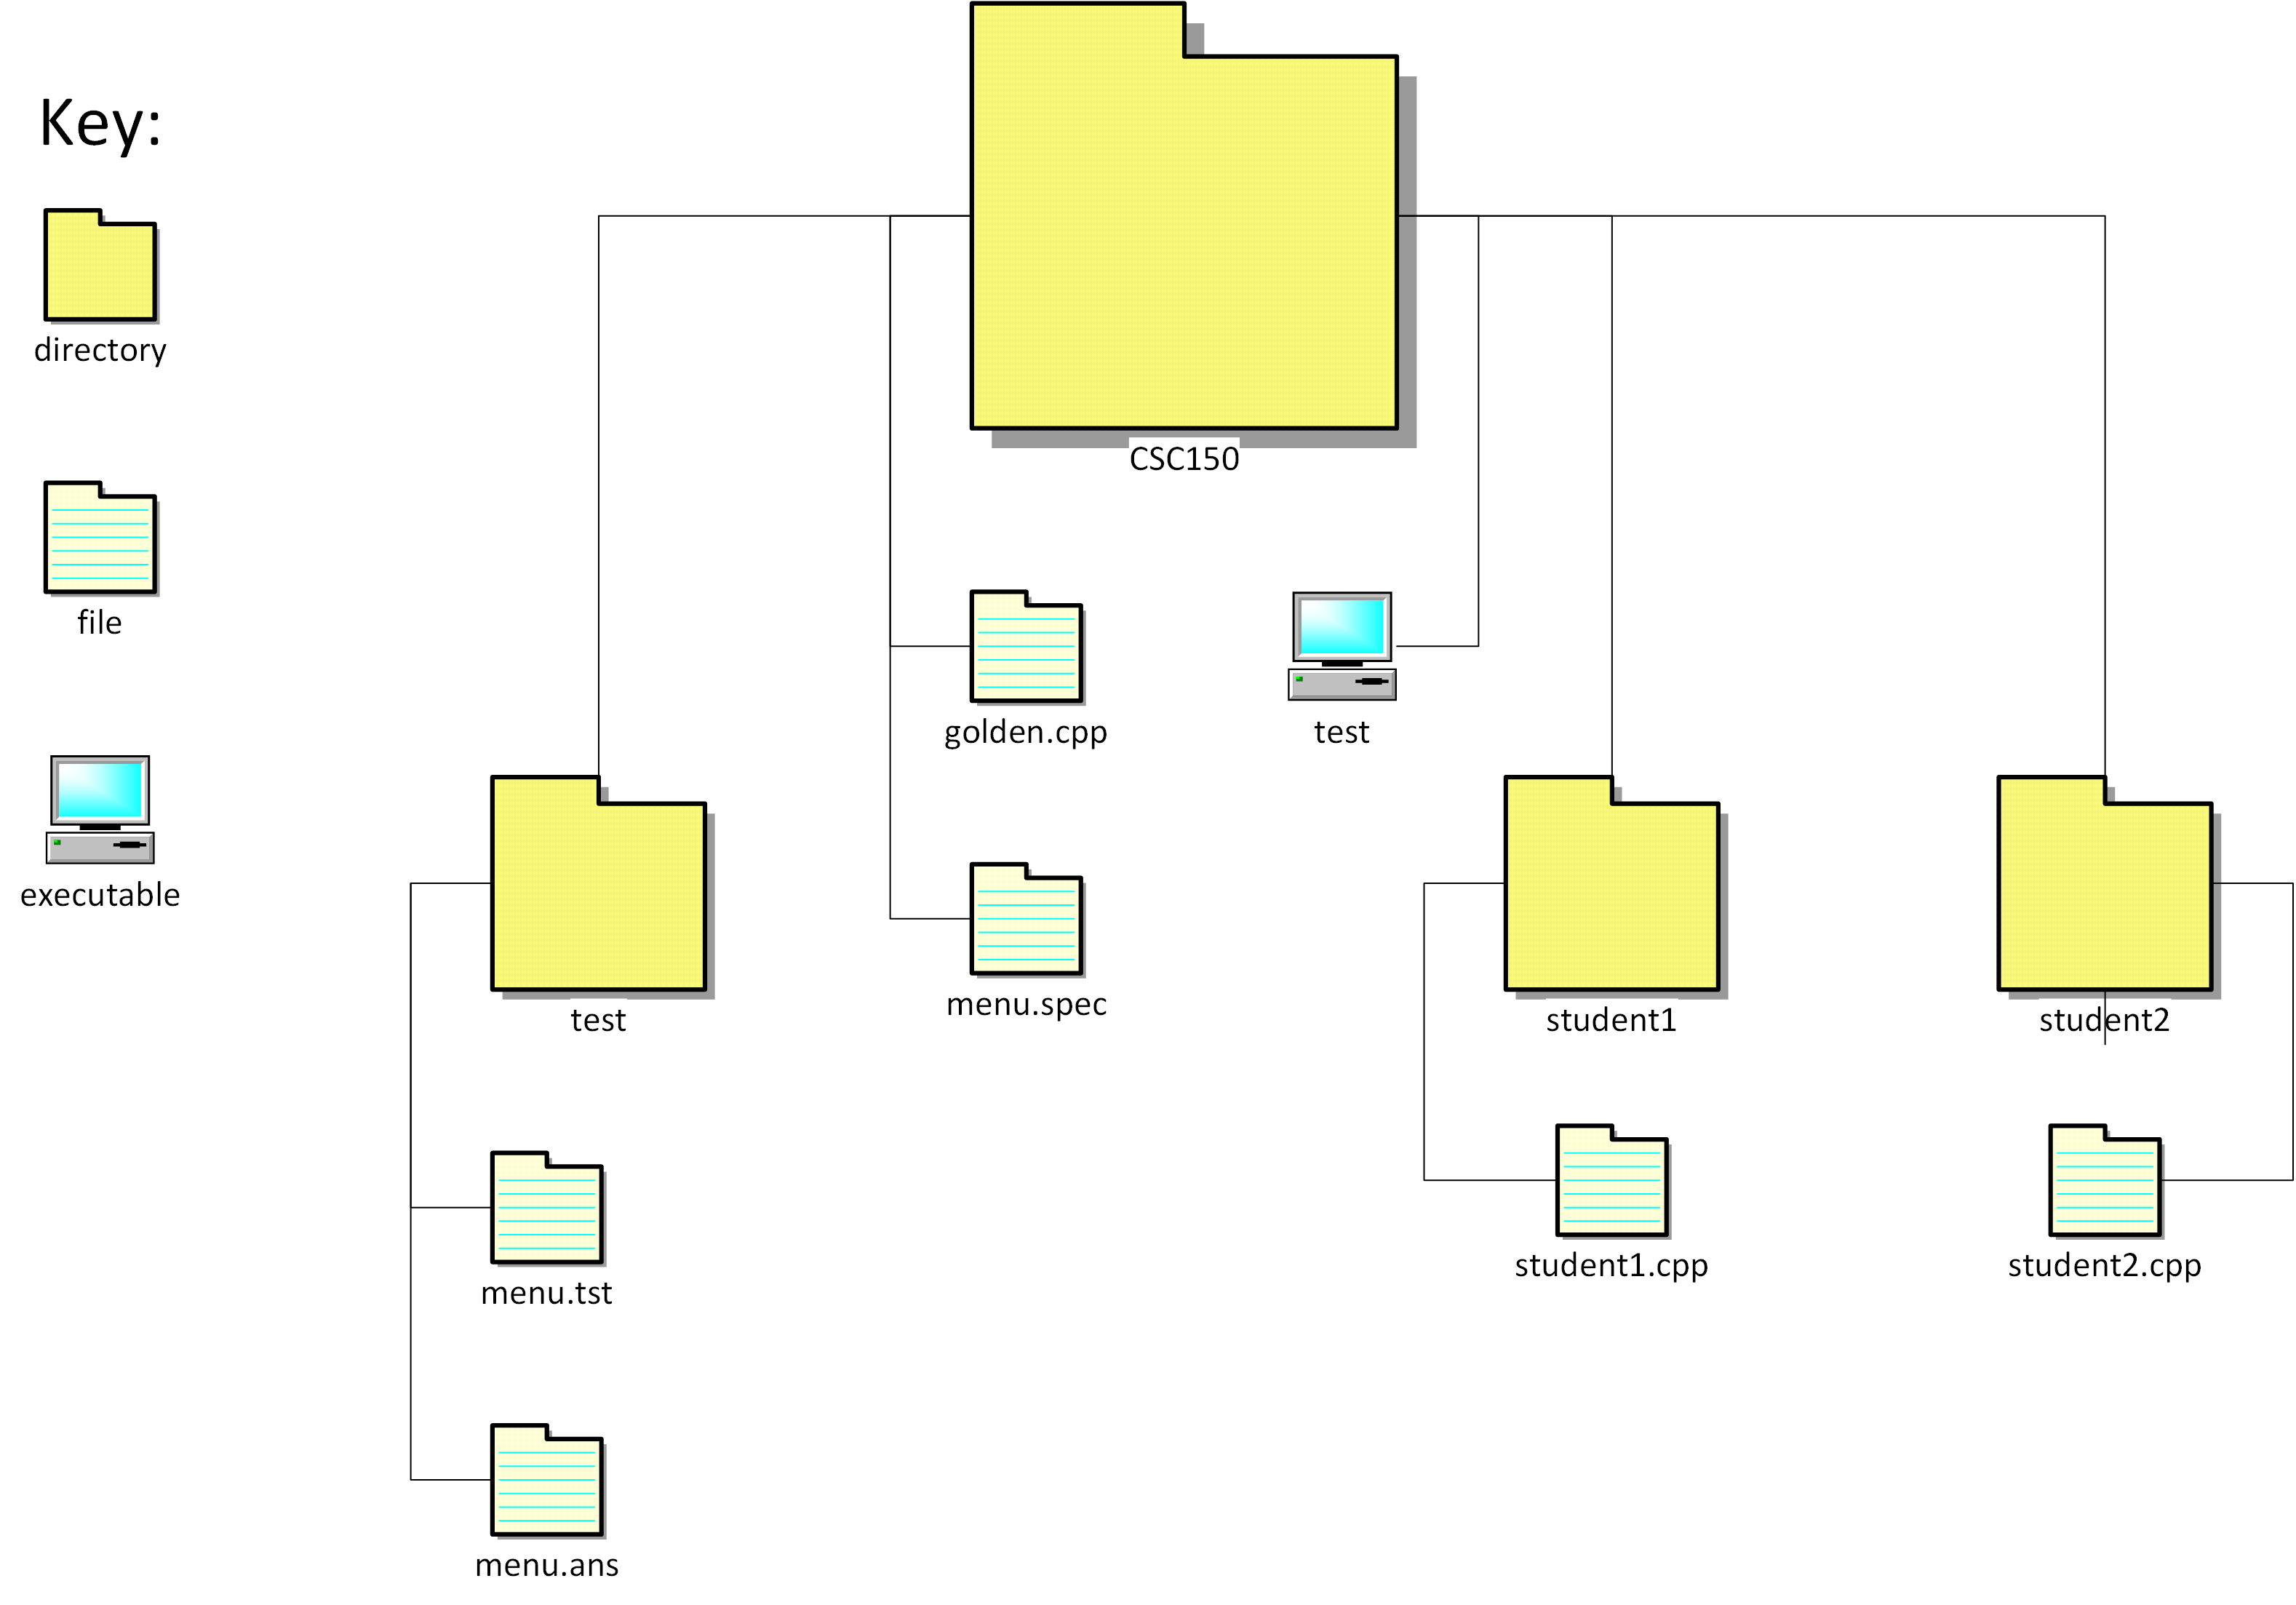
\includegraphics[width=0.75\textwidth]{./before}
\end{center}
\caption{Before test execution \label{before}}
\end{figure}

After the program, several more files have been added. The GeneratedTests directory has been created inside of test, and contains two .tst files and corresponding .ans files. In each student directory, an executable, a log file, .gprof and .gcov files, and gmon.out (created by gprof) have been added. In the parent directory, a class log has been created sharing the name of the directory. Figure ~\ref{after} shows the ending directory structure.

\begin{figure}[tbh]
\begin{center}
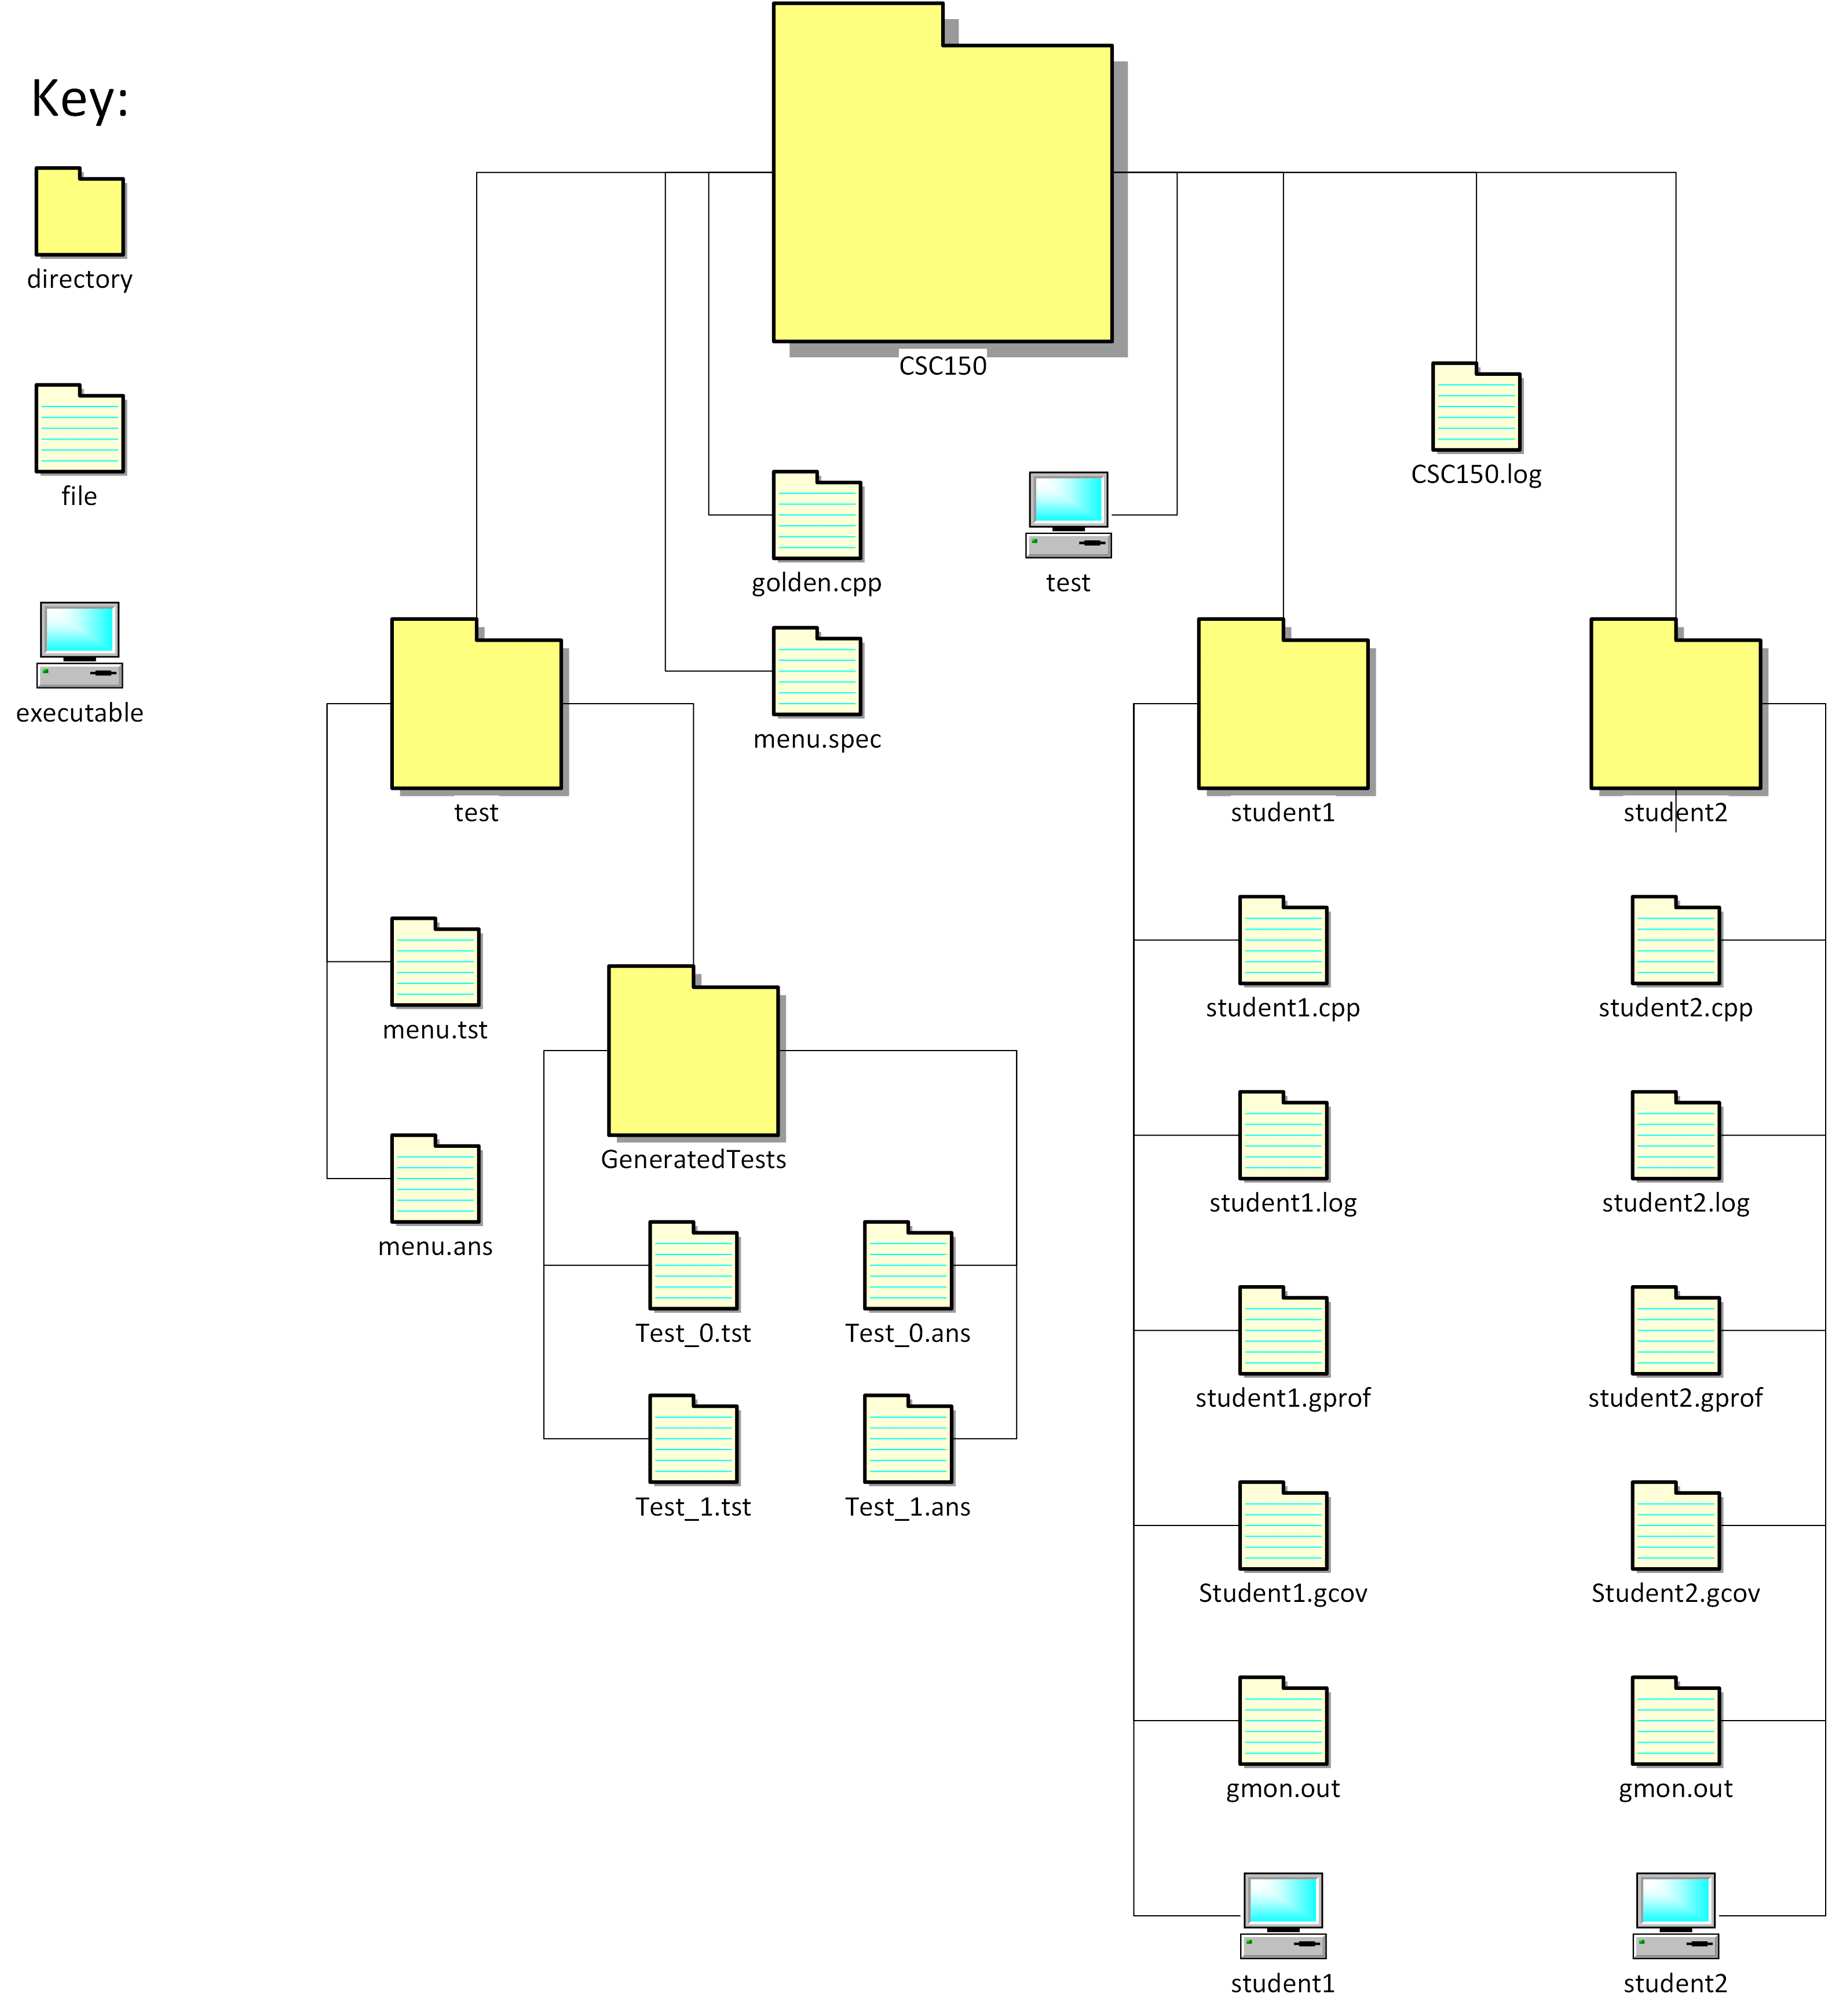
\includegraphics[width=0.75\textwidth]{./after}
\end{center}
\caption{After test execution \label{after}}
\end{figure}
% !TEX root = SystemTemplate.tex
\chapter{Development Environment}
This section will provide all the neccessary information to run, test and develop 
our source code.


\section{Development IDE and Tools}
The code was written in simple text editors, and requires no special IDE's or tools.  All
the code was tested on a Linux machine using the g++ compiler.  The debug tool
gdb was used to debug the code when necessary.

\section{Source  Control}
We used GitHub for source control.  The private repository can be found at this url: 

https://github.com/jcmanke/SoftEng/Sprint3.git

\section{Dependencies}
This program is dependent on the C++ Standard Library as well as the g++ compiler
on a Linux system.

\section{Build  Environment}
The execuatble is built by the g++ compiler.  You can either compile it manually, using the command:
\begin{lstlisting}
g++ -o test ProgramTester.cpp
\end{lstlisting}
Or by using the following make file:

\begin{lstlisting}
# compiler
CC = g++

# compiler options
CFLAGS = -c

#OBJECT FILES
OBJS = ProgramTester.cpp

tester: ProgramTester.cpp

	${CC} -g -lm ${OBJS} -o test
\end{lstlisting}

\section{Development Machine Setup}
For the Development Machine set up any Linux machine with the GNU compiler should work.


% !TEX root = SystemTemplate.tex

\chapter{Release -- Setup -- Deployment}
The source code will be provided to Dr. Logar using email or the Submit It! page of
the SDSMT Math and Computer Science webpage.


\section{Deployment Information and Dependencies}
Will need g++ and a linux like environment to run our program.


\section{Setup Information}
By navigating to the directory and running make, the program will be installed.


\section{System  Versioning Information}
The system is in 3.0.0 stage, or second release.

\input{userdocs.tex}


\backmatter
\chapter{Acknowledgement}
\label{SpecialThanks}  Thanks to Dr. Logar, for her help, knowledge and guidance.

\input{supporting.tex}
%%% Since counters are different in the backmatter section
%%% we explicitly set the section number  (comment out to see effect)
\setcounter{section}{0}
% !TEX root = SystemTemplate.tex

\chapter{Sprint Reports}

\section{Sprint Report \#1}
The testing function can traverse a directory looking for source code. Compile that code, then
look for test cases and run the compiled code with the given test case outputting the result in a 
new document. It can then compare that document with the expected results document and write
to the log file if it passed or failed. Then it will continue looking for test cases until all the test cases
in the root folder have been found. The tester will then write the total number of test cases passed,
total failed and the percentage passed and failed.

\section{Sprint Report \#2}

Had to redo a lot of the code. Most of it wasn't split into seperate functions and some of it was
misdocumented. After getting around that, we got it to travese the root directory, finding the
student directories and testing them against the tests located in the test directory. It can generate random
tests (the number of and data types specified by the user). Introduced a simple menu system to make it easier
to generate then run tests. It will log the results of the testing each student into a student log located in their
directory, and to a class log located in the root directory.

\section{Sprint Report \#3}

This section required a long time before we were even able to make it run. We used the test directory supplied on
the website, and the program would register a segmentation fault. It turns out that the previous group had
decided that all tests that were to be run would only be in a directory called tests, that the student directories
would only have one .cpp file and no files that contained cpp, such as a cpp.log. This also applied to the golden.cpp
that was expected to be the only cpp in the root testing directory.

After fighting through these issues, we managed to apply the new functionalities in short order. We implemented a
customized diff function for the new cases, added string generation to the menu, and implemented performance
testing and code coverage statistics through Gcov and Gprof. We also added a way to test if something was looping
for too long, with an option to change the default timeout after selecting to run tests. 

\input{industrial.tex}


\end{document}
